\documentclass[
  BCOR12mm,
  letterpaper,
  11pt,
  headsepline,
  pointlessnumbers,
  tablecaptionabove,
  headinclude,
  appendixprefix,
  idxtotoc,
  bibtotoc,
  twoside,
  titlepage
]{scrartcl}

% Fonts
\usepackage{mathptmx} % Times font in main text and mathematical formulas
\usepackage{wasysym}  % Contains several special symbols
\usepackage{pifont}   % Enables Zapf dingbats (special symbols)
\usepackage[scaled=.95]{helvet} % Sans serif font to be used

% Page style

\usepackage[automark]{scrpage2}
\usepackage[paper=letterpaper, centering]{geometry}

% Language definition
\usepackage[english]{babel}
\usepackage{varioref} % better references with \vref
\usepackage{natbib}   % nice citeation

% Figures
\usepackage{graphicx}
\usepackage{sidecap}
\usepackage{rotating}    % Allows setting sideways tables and figures, and to
                                        % rotate text.

% Some color in the document
\usepackage{color}

% Source code and pseudo code
\usepackage{listings}    % Source code listing support
\usepackage{algorithm}
\usepackage{algorithmic} % Algorithmen im Pseudo-Code,

\usepackage[unicode]{hyperref}
\usepackage[htt]{hyphenat}

% some nice colors
\definecolor{royalblue}{cmyk}{.93, .79, 0, 0}
\definecolor{lightblue}{cmyk}{.10, .017, 0, 0}
\definecolor{darkgreen}{rgb}{0,.7,0}
\definecolor{darkred}{rgb}{.7,0,0}
\definecolor{lightgray}{gray}{0.97}

% Style definitions

\selectlanguage{english}
\addtokomafont{sectioning}{\color{royalblue}}
\pagestyle{scrheadings}
\ifoot{
\includegraphics[width=50pt]{logo/JSBML_shaddow.pdf}}

\hypersetup{
              bookmarks={true},
              bookmarksopen={true},
              bookmarksopenlevel={0},
              bookmarksnumbered={true},
              breaklinks={true},
              colorlinks={false},
              pdfpagemode={UseOutlines},
              pdftitle={A short description of the main differences between
              JSBML and LibSBML},
              pdfauthor={Andreas Dr\"ager},
              pdfsubject={Software guide},
              pdfkeywords={LibSBML, JSBML, Java, SBML, API, LaTeX},
              pdfview={FitV},
              pdftex,
              pdffitwindow={true},
              pdfstartview={FitV},
              pdfnewwindow={false},
              pdfdisplaydoctitle={true},
              pdfhighlight={/P},
              plainpages={false},
              unicode={true},
              urlcolor={blue}
}

\lstset{language=Java,
captionpos=b,
basicstyle=\footnotesize\ttfamily\bfseries,
stringstyle=\color{darkred}\footnotesize\ttfamily,
keywordstyle=\color{royalblue}\bfseries\ttfamily,
ndkeywordstyle=\color{darkgreen},
numbers=left,
numberstyle=\footnotesize,
% backgroundcolor=\color{lightgray},
breaklines=true,
tabsize=2,
frame=single,
breakatwhitespace=true
% framexleftmargin=5mm,
% rulesepcolor=\color{lightgray}
% frameround=ttff
}

\hyphenation{
Cell-De-sig-n-er
}

\title{A short description of the main differences between JSBML and LibSBML}
\author{Andreas Dr\"ager\thanks{Center for Bioinformatics T\"ubingen, University
of T\"ubingen, T\"ubingen, Germany}\and%
Nicolas Rodriguez\thanks{European Bioinformatics Institute, Wellcome Trust
Genome Campus, Hinxton, Cambridge, United Kingdom}}
\date{\today}
\publishers{
\includegraphics[width=100pt]{logo/JSBML_shaddow.pdf}}

\begin{document}

\maketitle
\tableofcontents

\begin{abstract}
Although the libraries JSBML and LibSBML for working with files and data
structures defined in the standard SBML (Systems Biology Markup Language) are
very similar and share a common scope, users should be informed about their
major differences to switch from one library from the other one more easily. To
this end, the document at hand gives a brief overview of the main differences
between the Java\texttrademark{} application programming interfaces of both
libraries.

In addition, JSBML can be used as a communication layer between the widely
spread application CellDesigner and an application that works with JSBML as its
internal data structure. This document gives an example that demonstrates how to
convert between CellDesigner's plug-in data structures and JSBML objects.
\end{abstract}

\section{An extended type hierarchy}

Whenever multiple elements defined in the SBML specification share some
attributes, JSBML provides a common super class or at least a common interface
that gathers methods for manipulation of the shared properties. In this way, the
type hierarchy of JSBML has become more complex (see
Fig.~\vref{fig:TypeHierarchy}).
\begin{sidewaysfigure}[htbp]
\centering
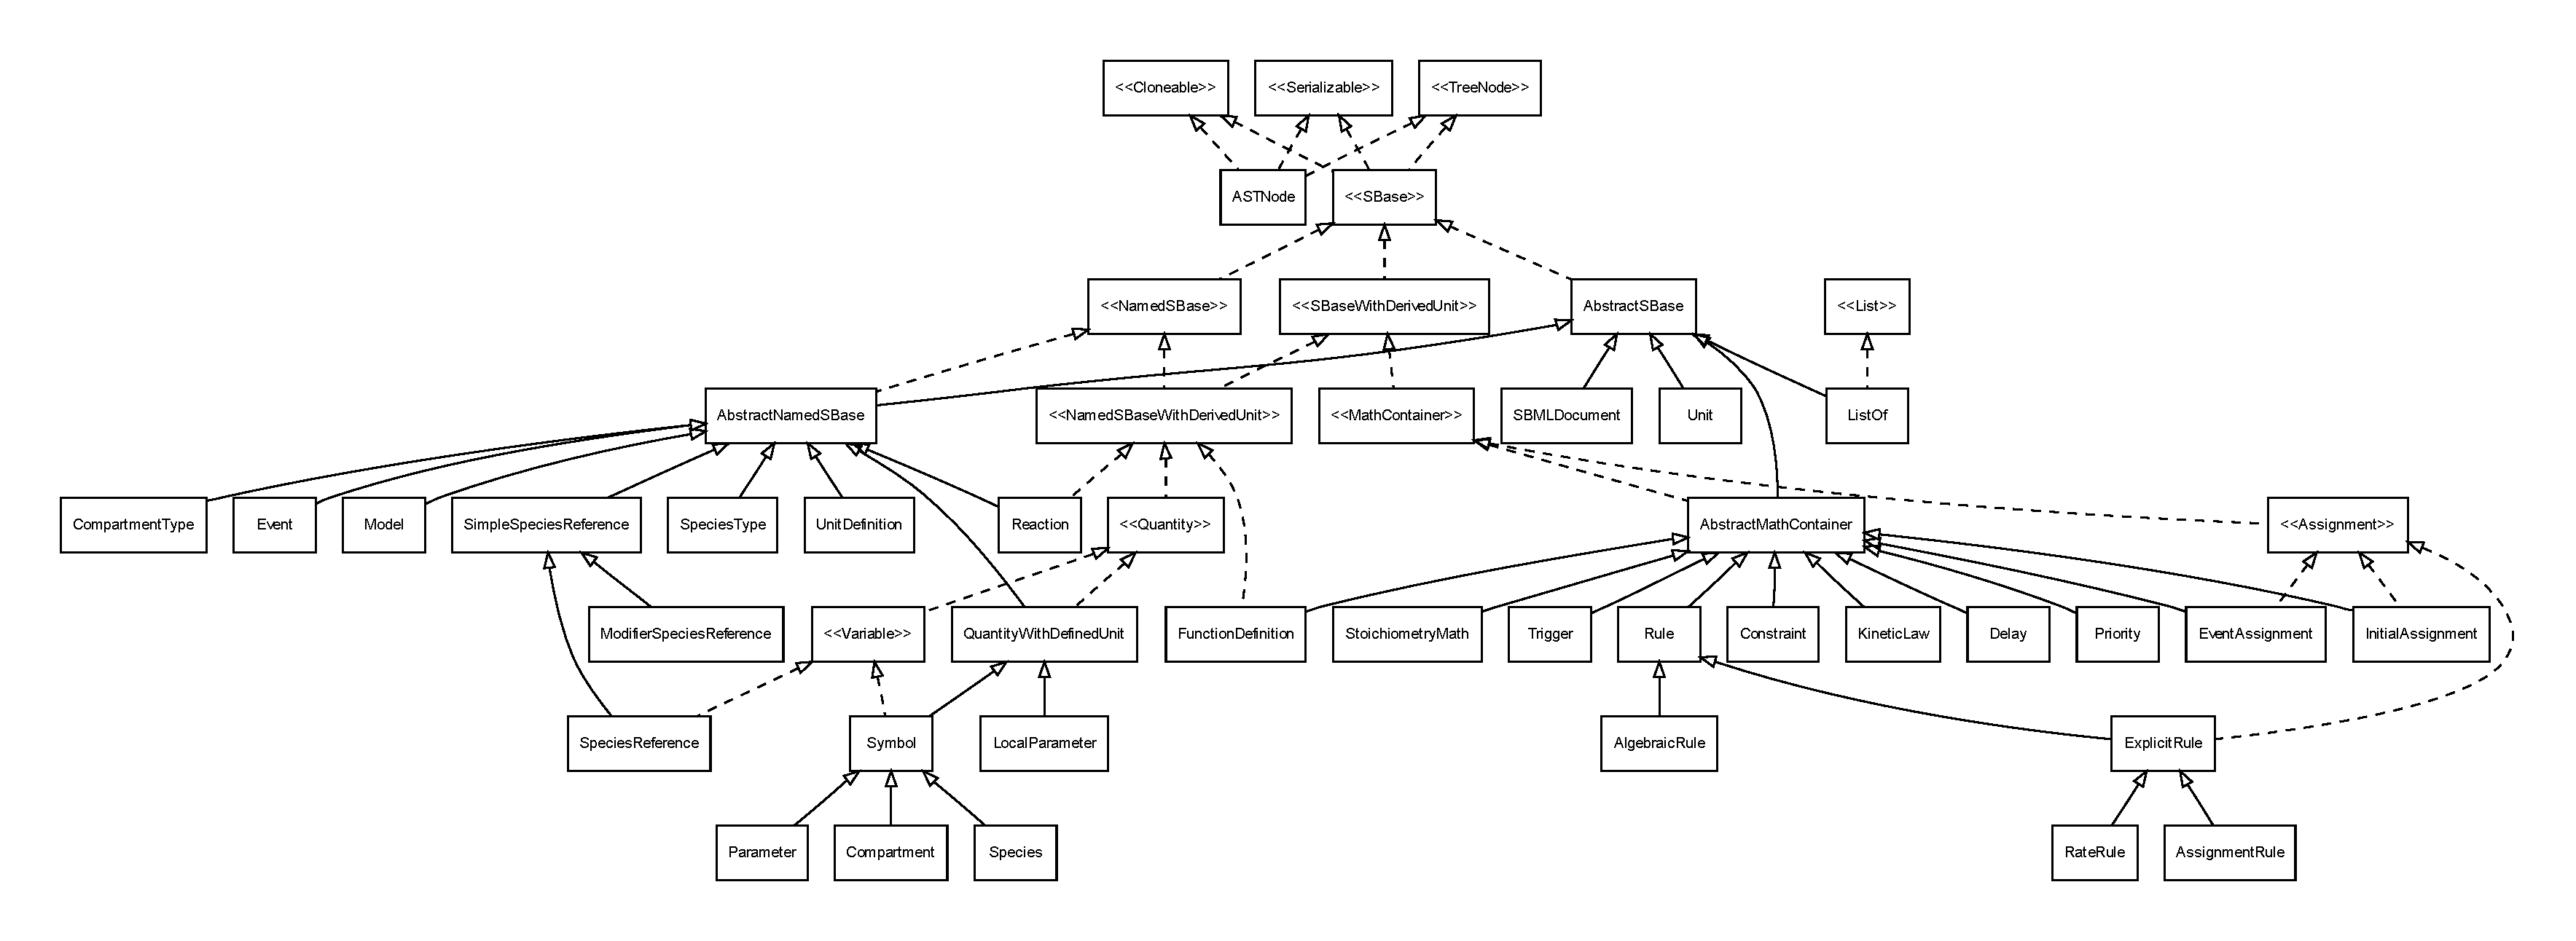
\includegraphics[width=\textwidth]{FullTypeHierarchy.pdf}
\caption[The type hierarchy in JSBML]{The type hierarchy of the main SBML
constructs in JSBML}
\label{fig:TypeHierarchy}
\end{sidewaysfigure}
Just like in LibSBML, all elements extend the abstract type \verb!SBase!, but in
JSBML, \verb!SBase! has become an interface. This allows more complex relations
between derived data types. In contrast to LibSBML, \verb!SBase! in JSBML
extends three other interfaces: \verb!Cloneable!, \verb!Serializable!, and
\verb!TreeNode!. As all elements defined in JSBML override the \verb!clone()!
method from the class \verb!java.lang.Object!, all JSBML elements can be deeply
copied and are therefore ``cloneable". By extending the interface
\verb!Serializable!, it is possible to store JSBML elements in binary form
without explicitly writing it to an SBML file. In this way, programs can easily
load and save their in-memory objects or send complex data structures
through a network connection without the need of additional file encoding and
subsequent parsing. The third interface, \verb!TreeNode! is actually defined in
Java's \verb!swing! package, but defines a data type independent of any
graphical information. It basically defines recursive methods on hierarchically
structured data types, such as iteration over all of its successors. In this
way, all instances of JSBML's \verb!SBase! interface can be directly passed to
the \verb!swing! class \verb!JTree! and hence be easily visualized.
Listing~\vref{lst:Visualization} demonstrates in a simple code example how to
parse an SBML file and to immediately display its content on a \verb!JFrame!.
\lstinputlisting[language=Java,float,caption={Parsing and visualizing the
content of an SBML file},label=lst:Visualization]{posters/2010_ICSB_and_COMBINE/JSBMLvisualizer.java}
Fig.~\vref{fig:Visualization} shows an example output when applying the program
from Listing~\vref{lst:Visualization} to SBML test model \texttt{case00026}.
\begin{SCfigure}[][t]
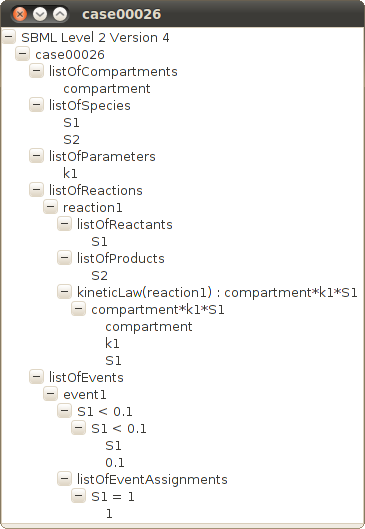
\includegraphics[width=.35\textwidth]{posters/2010_ICSB_and_COMBINE/JSBMLvisualizerTransparent}
\caption[Tree representation of an SBML file]{A tree representation of the
content of SBML test model \texttt{case00026}}
\label{fig:Visualization}
\end{SCfigure}
The \verb!ASTNode! class in JSBML also implements all these three interfaces and
can hence be cloned, serialized, and visualized in the same way.


\subsection{The \texttt{Assignment} class}

JSBML unifies all those elements that assign values to some other
\verb!SBase! in SBML under the interface \texttt{Assignment}. This interface
uses the term Variable for the element whose value is to be changed depending
on some mathematical expression that is also present in the Assignment
(because Assignment extends the interface \texttt{MathContainer}). Therefore,
an Assignment contains methods such as
\verb!set!-/\verb!getVariable(Variable v)! and also \verb!isSetVariable()! and
\verb!unsetVariable()!. In addition to that JSBML also provides the method \verb!set!-/\verb!getSymbol(String symbol)! in the \texttt{InitialAssignment}
class to make sure that switching from LibSBML to JSBML is quite smoothly.
However, the preferred way in JSBML is to apply the methods
\texttt{setVariable} either with String or Variable instances as arguments.

\subsection{The \texttt{MathContainer} interface}

This interface gathers all those elements that may contain mathematical
expressions encoded in abstract syntax trees (instances of \verb!ASTNode!).
The abstract class \verb!AbstractMathContainer! serves as actual super class
for most of the derived types.



\section{Abstract syntax trees}

Both libraries define a class \verb!ASTNode! for in-memory manipulation and
evaluation of abstract syntax trees that represent mathematical formulas and
equations. These can either be parsed from a representation in \verb!C!
language-like \verb!String!s, or from a MathML representation. The JSBML
\verb!ASTNode! provides various methods to transform these trees to other
formats, for instance, \LaTeX{} \verb!String!s. In JSBML, several static methods
allow easy creation of new syntax trees, for instance, the following code
\begin{verbatim}
ASTNode myNode = ASTNode.plus(myLeftAstNode, myRightASTNode);
\end{verbatim}
creates a new instance of \verb!ASTNode! which represents the sum of the two
other \verb!ASTNode!s. In this way, even complex trees can be easily
manipulated.

\section{The \texttt{ASTNodeCompiler} class}

This interface allows users to create customized interpreters for the
content of mathematical equations encoded in abstract syntax trees. It
is directly and recursively called from the \verb!ASTNode! class and returns
an \verb!ASTNodeValue! object, which wraps the possible evaluation results of
the interpretation. JSBML already provides several implementations of
this interface, for instance, \verb!ASTNode! objects can be directly translated
to LaTeX or MathML for further processing.

\section{Cloning when adding child nodes}

When adding elements such as a \verb!Species! to a \verb!Model!, LibSBML will
clone the object and add the clone to the \verb!Model!. In contrast, JSBML does
not automatically perform cloning. The advantage is that modifications on the
object belonging to the original pointer will also propagate to the element
added to the \verb!Model!. Furthermore, this is more efficient with respect to
the run time and also more intuitive. If cloning is necessary, users should call
the \verb!clone()! method manually. Since all instances of \verb!SBase! and also
\verb!Annotation!, \verb!ASTNode!, \verb!CVTerm!, and \verb!History! implement
the interface \verb!Cloneable! (see Fig.~\vref{fig:TypeHierarchy}), all these
elements can be naturally cloned. However, when cloning an object in JSBML, such
as an \verb!AbstractNamedSBase!, all children of this element will be cloned
before adding them to the new element. This is necessary, because the data
structures specified in SBML define a tree, in which each element has exactly
one parental node.


\section{Change events and listeners}

JSBML introduces the possibility to listen to change events in the life of an
SBML document. To benefit from this advantage, simply let your class implement
the interface \verb!SBaseChangeListener! and add it to the list of listeners in
your instance of  \verb!SBMLDocument!. You only have to implement three methods
\begin{description}
 \item[sbaseAdded] This method notifies the listener that the given \verb!SBase!
   has just been added to the \verb!SBMLDocument!
 \item[sbaseRemoved] The \verb!SBase! instance passed to this method is no
   longer part of the \verb!SBMLDocument! as it has just been removed.
 \item[stateChanged] This method provides detailed information about some value
   change within the \verb!SBMLDocument!. The object passed to this method is
   an \verb!SBaseChangeEvent!, which provides information about the \verb!SBase!
   that has been changed, its property whose value has been changed (this is a
   \verb!String! representation of the name of the property), along with the
   previous value and the new value.
\end{description}
With the help of these methods, you can keep track of what your
\verb!SBMLDocument! does at any time. Furthermore, one could consider to make
use of this functionality in a graphical user interface, where the user should
be asked if he or she really wants to delete some element or to approve changes
before making these persistent. Another idea of using this, would be to write
log files of the model building process automatically.


\section{Deprecation}

The intension of JSBML is to provide a Java library for the latest 
specification of SBML. Hence, JSBML provides methods and classes to
cover earlier releases of SBML as well, but these are often marked
as being deprecated to avoid creating models that refer to these 
elements.

\section{Exceptions}

Generally, JSBML throws more exceptions than LibSBML. This behavior helps
programmers and users to avoid creating invalid SBML data structures already
when dealing with these in memory. Examples are the \verb!ParseException! that
may be thrown if a given formula cannot be parsed properly into an
\verb!ASTNode! data structure, or \verb!InvalidArgumentException!s if
inappropriate values are passed to methods. For instance, an object representing
a constant such as a \verb!Parameter! whose constant attribute has been set to
\verb!true! cannot be used as the \verb!Variable! element in an
\verb!Assignment!. Another example is the \verb!InvalidArgumentException! that
is thrown when trying to set an invalid identifier \verb!String! for an instance
of \verb!AbstractNamedSBase!. Hence, you have to be aware of potential
exceptions and errors when using JSBML, on the other hand this will 
prevent you from doing obvious mistakes.


\section{Model history}

In earlier versions of SBML only the model itself could be associated with a
history, i.e., a description about the person(s) who build this model, including
names, e-mail addresses, modification and creation dates. Nowadays, it has
become possible to annotate each individual construct of an SBML model with such
a history. This is reflected by naming the corresponding object \verb!History!
in JSBML, whereas it is still called \verb!ModelHistory! in LibSBML. Hence, all
instances of \verb!SBase! in JSBML contain methods do access and manipulate its
\verb!History!. Furthermore, you will not find the classes \verb!ModelCreator!
and \verb!ModelCreatorList! because JSBML gathers its \verb!Creator! objects
in a generic \verb!List<Creator>! in the \verb!History!.
 

\section{The classes \texttt{libSBML} and \texttt{JSBML}}

There is no class \texttt{LibSBML} because this library is called
\texttt{JSBML}. You can therefore only find a class \texttt{JSBML}. This class
provides some similar methods as the \texttt{LibSBML} class in LibSBML, such as
\verb!getJSBMLDottedVersion()! to obtain the current version of the JSBML
library. However, many other methods that you might expect to find there, if you
are used to LibSBML, are located in the actual classes that are related with the
function. For instance, the method to convert between a \verb!String! and a
corresponding \verb!Unit.Kind! can be done by using the method
\begin{verbatim}
Unit.Kind.valueOf(myString);
\end{verbatim}
In a similar way, the \verb!ASTNode! class provides a method to parse C-like
formula \verb!String!s according to the specification of SBML Level 1 into an
abstract syntax tree. Therefore, in contrast to the  \texttt{LibSBML} class, the
class \texttt{JSBML} contains only a few methods.


\section{Replacement of the interface \texttt{libSBMConstants} by Java enums}

You won't find a corresponding implementation of this interface in 
JSBML. The reason is that the JSBML team decided to encode constants using the
Java construct enum. For instance, all the fields starting with the
prefix \verb!AST_TYPE_*! have a corresponding field in the \verb!ASTNode! class
itself. There you can find the Type enum. Instead of typing
\verb!AST_TYPE_PLUS!, you would therefore type \verb!ASTNode.Type.PLUS!.

The same holds true for \verb!Unit.Kind.*! corresponding to the 
\verb!LibSBMLConstants.UNIT_KIND_*! fields.


\section{Various types of \texttt{ListOf*} classes}

There is no method \verb!get(String id)! because the generic implementation of 
the \verb!ListOf<? extends SBase>! class in JSBML excepts also elements that do 
not necessarily have an identifier. Only instances of \verb!NamedSBase! may have
the fields identifier and name set. Hence, generally, the \verb!ListOf! class 
cannot assume these fields to be present. To query an instance of \verb!ListOf! 
in JSBML for names or identifiers or both, you can apply the following filter:
\begin{verbatim}
NamedSBase nsb = myList.firstHit(new NameFilter(identifier));
\end{verbatim}
This will give you the first element in the list with the given identifier.
Various filters are already implemented, but you can easily add your 
customized filter. To this end, you only have to implement the \verb!Filter! 
interface in \verb!org.sbml.jsbml.util.filters!. There you can also find an
\verb!OrFilter! and an \verb!AndFilter!, which take as arguments multiple other
filters. With the \verb!SBOFilter! you can query for certain SBO annotations in
your list, whereas the \verb!CVTermFilter! helps you to identify \verb!SBase!
instances with a desired MIRIAM annotation. For instances of
\verb!ListOf<Species>! you can apply the \verb!BoundaryConditionFilter! to look
for those species that operate on the boundary of the reaction system.


\section{Units}

Since SBML Level 3 the data type of the exponent attribute in the \verb!Unit!
class has been changed from \verb!int! to \verb!double! values. JSBML reflects
this in the method \verb!getExponent()! by returning \verb!double! values only.
For a better compatibility with LibSBML, whose corresponding method still
returns \verb!int! values, JSBML also provides the method
\verb!getExponentAsDouble()!. This method returns the value from the
\verb!getExponent()! method and is therefore absolutely redundant.

\section{Unit Definitions}

\subsection{Predefined unit definitions}

A model in JSBML always also contains all predefined units in the model
if there are any, i.e., for models encoded of SBML versions before level
3. These can be accessed from an instance of model by calling the method
\verb!getPredefinedUnit(String unit)!.

\subsection{Access to the units of an element}

In JSBML, all SBML elements that can be associated with some unit implement the
interface \verb!SBaseWithUnit!. This interface provides methods for direct
access to an object representing their unit. Currently, the following elements
implement this interface:
\begin{itemize}
 \item \verb!AbstractNamedSBaseWithUnit!
 \item \verb!ExplicitRule!
 \item \verb!KineticLaw!
\end{itemize}
Fig.~\vref{fig:TypeHierarchy} provides a better overview about the relationships
between all the classes explained here.
Note that \verb!AbstractNamedSBaseWithUnit! serves as the abstract super class
for \verb!Event! and \verb!QuantityWithUnit!. In \verb!Event!, all methods to
deal with units are already deprecated because only in SBML Level 1 Versions 1
and 2 \verb!Event!s could be explicitly equipped with units. The same holds true
for instances of \verb!ExplicitRule! and \verb!KineticLaw!, which both can only
explicitly be populated with units for SBML in Level 1, Version 1 and 2. In
contrast, \verb!QuantityWithUnit! serves as the abstract super class for
\verb!LocalParameter! and \verb!Symbol!, which is then again the super type of
\verb!Compartment!, \verb!Species!, and (global) \verb!Parameter!.

Care must be taken when obtaining an instance of \verb!UnitDefinition! from one
of the classes implementing \verb!SBaseWithUnit!
because it might happen that the given \verb!UnitDefinition! has just been
created for convenience from the information provided by the class, but that the
model containing this \verb!SBaseWithUnit! does actually not contain this
\verb!UnitDefinition!. It might therefore be useful to either check if the
\verb!Model! contains this \verb!UnitDefinition! or to add it to the
\verb!Model!.

In case of \verb!KineticLaw! it is even more difficult, because
SBML Level 1 allows to separately set the substance unit and the time unit of
the element. To unify the API, we decided to also provide methods that allow
the user to simply pass one \verb!UnitDefinition! or its identifier to
\verb!KineticLaw!. These methods then try to guess if a substance unit or time
unit is given. Furthermore, it is possible to pass a \verb!UnitDefinition!
representing a variant of substance per time directly. In this case, the
\verb!KineticLaw! will memorize a direct link to this \verb!UnitDefinition! in
the model and also try to save separate links to the time unit and the substance
unit. However, this may cause a problem if the containing \verb!Model! does not
contain separate \verb!UnitDefinition!s for both enties.

Generally, this approach provides a more general way to access and manipulate
units of SBML elements.

\appendix

\section{Frequently Asked Questions (FAQ)}


\subsection{Why does the class \texttt{LocalParameter} not inherit from
\texttt{Parameter}?}

The reason is the Boolean attribute \texttt{constant}, which is present in
\texttt{Parameter} and can be set to \texttt{false}. A parameter in the meaning
of SBML is not a constant, it might be some system variable and can therefore
be the subject of \texttt{Rule}s, \texttt{Event}s and to on, whereas a
\texttt{LocalParameter} is defined as a constant quantity that never changes its
value during the evaluation of a model. It would therefore only be possible to
let \texttt{Parameter} inherit from \texttt{LocalParameter} but this could lead
to a semantic misinterpretation.


\section{An example of how to turn a JSBML-based application into a CellDesigner
plug-in}

Once an application has been implemented based on JSBML, it can easily be
accessed from CellDesigner's plug-in menu \citep{Funahashi2003}. To this end,
it is necessary to extend two classes that are defined in CellDesigner's plug-in
API (Abstract Programming Interface). The
Listings~\vrefrange{lst:PluginAction}{lst:Plugin} show a very simple example of
how to pass CellDesigner plug-in model data structures to the translator in
JSBML, which creates then a JSBML \verb!Model! data structure.
\lstinputlisting[language=Java,float,caption={A simple implementation of
CellDesigner's abstract class \texttt{PluginAction}},
label=lst:PluginAction]{SimpleCellDesignerPlugin/org/sbml/jsbml/cdplugin/SimpleCellDesignerPluginAction.java}
% \lstinputlisting[language=Java,float,caption={SimpleCellDesignerPlugin},
% label=lst:Plugin]{SimpleCellDesignerPlugin/org/sbml/jsbml/cdplugin/SimpleCellDesignerPlugin.java}
\begin{lstlisting}[language=Java,float,caption={A simple example for a
CellDesigner plug-in using JSBML as a communication layer},label=lst:Plugin]
package org.sbml.jsbml.cdplugin;

import javax.swing.*;
import jp.sbi.celldesigner.plugin.*;
import org.sbml.jsbml.*;
import org.sbml.jsbml.gui.*;

/** A very simple implementation of a plug-in for CellDesigner. */
public class SimpleCellDesignerPlugin extends CellDesignerPlugin {

  public static final String ACTION = "Display full model tree";
  public static final String APPLICATION_NAME = "Simple Plugin";

  /** Creates a new CellDesigner plug-in with an entry in the menu bar. */
  public SimpleCellDesignerPlugin() {
    super();
    try {
      System.out.printf("\n\nLoading %s\n\n", APPLICATION_NAME);
      SimpleCellDesignerPluginAction action = new SimpleCellDesignerPluginAction(this);
      PluginMenu menu = new PluginMenu(APPLICATION_NAME);
      PluginMenuItem menuItem = new PluginMenuItem(ACTION, action);
      menu.add(menuItem);
      addCellDesignerPluginMenu(menu);
    } catch (Exception exc) {
      exc.printStackTrace();
    }
  }

  /** This method is to be called by our CellDesignerPluginAction. */
  public void startPlugin() {
    PluginSBMLReader reader = new PluginSBMLReader(getSelectedModel(), SBO
        .getDefaultPossibleEnzymes());
    Model model = reader.getModel();
    SBMLDocument doc = new SBMLDocument(model.getLevel(), model
        .getVersion());
    doc.setModel(model);
    new JSBMLvisualizer(doc);
  }

  // Include also methods from super class, not needed in this example.
  public void addPluginMenu() { }
  public void modelClosed(PluginSBase psb) { }
  public void modelOpened(PluginSBase psb) { }
  public void modelSelectChanged(PluginSBase psb) { }
  public void SBaseAdded(PluginSBase psb) { }
  public void SBaseChanged(PluginSBase psb) { }
  public void SBaseDeleted(PluginSBase psb) { }
}
\end{lstlisting}
The example described by Listings~\vrefrange{lst:PluginAction}{lst:Plugin}
create a plug-in for CellDesigner, which displays the SBML data structure
in a tree, like the example in Fig.~\vref{fig:Visualization}. This example only
shows how to translate a plug-in data structure
from CellDesigner into a corresponding JSBML data structure. With the help of
the class \verb!PluginSBMLWriter! it is possible to notify CellDesigner about
changes in the model data structure. Note that Listing~\vref{lst:Plugin} is only
completed by implementing the methods from the super class. In this example it
is sufficient to leave the implementation open.

\bibliographystyle{natbib}
\bibliography{literature}

\end{document}
